\chapter{Observations, Rewards and Masks}\label{ch:obs}

The network is told almost nothing beyond the board itself. Its input is a stack of grids
describing the game from its own point of view. Its reward only says who won. One
mask removes moves that would kill it outright. This chapter defines all three.

\section{Eight egocentric planes}

\begin{defbox}[Observation]
For viewer $k$, the observation is a tensor $o^k\in[0,1]^{8\times B\times B}$. ``Own''
refers to snake $k$, ``enemy'' to every other living snake; dead snakes are invisible.
With body $x_0,\dots,x_{L-1}$:
\begin{center}
\begin{tabular}{@{}clp{0.56\linewidth}@{}}
\toprule
& \textbf{Plane} & \textbf{Value at a cell}\\
\midrule
0 & own head & $1$ at $x^k_0$\\
1 & own body & $1$ at $x^k_1,\dots,x^k_{L_k-1}$\\
2 & own age & $(L_k-i)/L_k$ at $x^k_i$: $1$ at the head, $1/L_k$ at the tail\\
3 & enemy heads & $1$ at every $x^j_0$, $j\ne k$\\
4 & enemy bodies & $1$ at every enemy non-head segment\\
5 & dangerous heads & $1$ at $x^j_0$ for enemies with $L_j \ge L_k$\\
6 & food & $1$ at every food cell\\
7 & health & $h_k/h_{\max}$ everywhere (0 if $k$ is dead)\\
\bottomrule
\end{tabular}
\end{center}
\end{defbox}

\begin{center}
\setlength{\tabcolsep}{4pt}
\begin{tabular}{@{}cccc@{}}
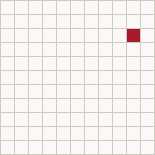
\includegraphics[width=0.22\linewidth]{figures/obs_own_head.png} &
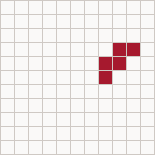
\includegraphics[width=0.22\linewidth]{figures/obs_own_body.png} &
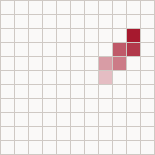
\includegraphics[width=0.22\linewidth]{figures/obs_own_age.png} &
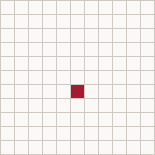
\includegraphics[width=0.22\linewidth]{figures/obs_enemy_heads.png}\\
\footnotesize own head & \footnotesize own body & \footnotesize own age & \footnotesize enemy heads\\[4pt]
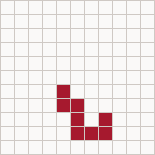
\includegraphics[width=0.22\linewidth]{figures/obs_enemy_bodies.png} &
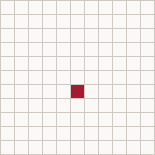
\includegraphics[width=0.22\linewidth]{figures/obs_danger.png} &
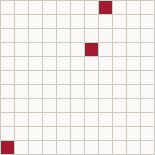
\includegraphics[width=0.22\linewidth]{figures/obs_food.png} &
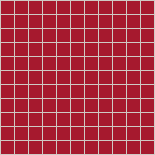
\includegraphics[width=0.22\linewidth]{figures/obs_health.png}\\
\footnotesize enemy bodies & \footnotesize dangerous heads & \footnotesize food & \footnotesize health
\end{tabular}
\captionof{figure}{The eight planes for the orange snake in the duel position of
Figure~\ref{fig:duel-board}. Shade is the plane's value: the age plane fades from head to
tail, and the health plane is uniform.}
\label{fig:obs-planes}
\end{center}

\begin{keybox}[Egocentric, not hand-engineered]
Every plane is a direct transcription of the board; nothing is computed that the rules do
not already state. The legacy agent's A* path quality and dead-end lookahead are gone.
Three design choices still matter:
\begin{itemize}
\item \textbf{Self versus others} rather than ``snake 0 versus snake 1''. Swapping two
  snakes swaps their observations, which is tested, so one network can play any seat.
\item \textbf{The age plane} tells the network which segment leaves next, which is how
  it can know a tail cell will be free.
\item \textbf{The dangerous-heads plane} restates the head-to-head rule
  (Chapter~\ref{ch:game}) in a form a convolution can read locally.
\end{itemize}
\end{keybox}

\begin{warnbox}[Segments that share a cell]
At the start all three segments of a snake share one cell, and after eating the tail is
duplicated. Planes are written tail-first, so where segments overlap the one nearest the
head wins. The duplicated tail cell therefore reads $2/L$ rather than $1/L$ on the
turn after eating, a deliberate and documented simplification.
\end{warnbox}

\section{Walls}

Nothing in the eight planes marks the edge of the board. The network supplies it itself:
it appends a constant plane of ones before the first convolution. Zero padding then
makes that plane drop to $0$ exactly outside the board, so every filter that touches the
edge can tell. This avoids an extra input plane that would be identical in every
position.

\section{The arena window}\label{sec:window}

A network whose first fully connected layer expects $64\cdot 11\cdot 11$ inputs is
bound to an $11\times11$ board. The arena network instead reads a fixed-size window
around its own head.

\begin{defbox}[Window observation]
For odd $W$ and viewer $k$ with head at $(r_0,c_0)$, the window observation is
$w^k\in[0,1]^{9\times W\times W}$ with
\[
  w^k_{c}(i,j) =
  \begin{cases}
    o^k_c\bigl(r_0 - \lfloor W/2\rfloor + i,\ c_0 - \lfloor W/2\rfloor + j\bigr)
      & \text{if that cell is on the board,}\\
    0 & \text{otherwise,}
  \end{cases}
\]
for the eight planes $c=0,\dots,7$, plus a ninth \emph{wall} plane equal to $1$ exactly
where the window extends past the board. The arena uses $W=17$ on a $19\times19$ board.
\end{defbox}

\begin{center}
\setlength{\tabcolsep}{6pt}
\begin{tabular}{@{}ccc@{}}
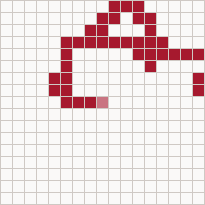
\includegraphics[width=0.27\linewidth]{figures/window_bodies.png} &
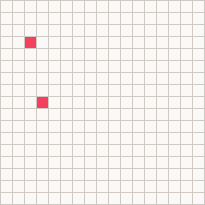
\includegraphics[width=0.27\linewidth]{figures/window_food.png} &
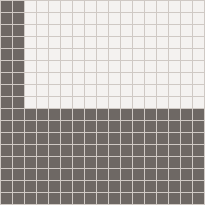
\includegraphics[width=0.27\linewidth]{figures/window_wall.png}\\
\footnotesize snakes (heads lighter) & \footnotesize food & \footnotesize wall plane
\end{tabular}
\captionof{figure}{The $17\times17$ window of one arena snake at turn 120, centred on its
head. The grey wall plane marks the part of the window that hangs off the board.}
\label{fig:window}
\end{center}

Because the window always sits on the snake's own head, its centre is always ``me''. The
same weights serve any board size and any number of opponents. The crop is fully
vectorised: row and column index grids are built from the head positions, clipped to the
board for the lookup, and multiplied by an in-bounds mask.

\section{Rewards}

\begin{defbox}[Reward functions]
\textbf{\code{winloss}} (default for $S>1$): $+1$ to the winner when the game ends,
$-1$ to a snake on the turn it dies, and $0$ to snakes that die together on the final
turn of a game with no winner.

\textbf{\code{food}} (default for $S=1$): $+1$ per food eaten, $-1$ on death.

\textbf{Training reward}: \code{winloss} plus a small shaping term,
\[
  r_t^k = R^k_t + 0.05\cdot\mathbf{1}[\,k \text{ ate at } t\,].
\]
\end{defbox}

The shaping bonus is twenty times smaller than a win, small enough that the agent never
prefers eating to winning. It is large enough to make early exploration find food before
it can find wins.

\section{Episode boundaries and padding}

With two snakes, a death ends the game. With six it does not, and a dead snake's seat
keeps producing ``transitions'' until the game ends. These are padding: its actions are
ignored and its rewards are zero.

\begin{defbox}[Dones and the active mask]
\[
  \text{done}^k_t = \text{died}^k_t \;\vee\; \text{game\_over}_t,
  \qquad
  \text{active}^k_t = \text{alive}^k_{t-1}\wedge \neg\,\text{over}_{t-1}.
\]
Every slot of a game that ends receives \emph{done}, so no slot's trajectory runs into the
next game. A transition is real only where \emph{active} holds, and the trainer masks
everything else out of the loss.
\end{defbox}

\begin{warnbox}[Found in review]
An earlier version set \emph{done} only for snakes alive at the end, so with three or more
snakes a dead seat never saw an episode boundary, and nothing marked its padding steps.
A probe of 64 games with 3 snakes over 400 turns counted 12{,}682 such zombie
transitions. Two-snake games were never affected, but the arena would have been. The
fix above landed before any multi-snake training.
\end{warnbox}

\section{The action mask}

\begin{defbox}[Action mask]
Let the \emph{blocked} cells be every segment of every living snake except its last,
since tails move away. Move $a$ is \emph{safe} for snake $k$ if
$x^k_0+\delta(a)$ is on the board and not blocked. A duplicated tail stays blocked
automatically, because its copy is the second-to-last segment.
\end{defbox}

The policy's logits for unsafe moves are set to $-10^9$ before the softmax, so the network
never wastes probability, or gradient, on walking into a wall. If no move is safe, all
four are allowed and the snake dies anyway. The mask is deliberately optimistic in two
ways that the network must learn to handle itself:
\begin{itemize}
\item it assumes enemy tails move, so it cannot know that an enemy is about to eat and
  keep its tail where it is;
\item it ignores head-to-head risk, which the dangerous-heads plane exposes instead.
\end{itemize}
